\chapter{概率图模型概述}
\label{chap:pgm-overview}

一台设备发出报警，是否应当立即停机？报警可能来自设备故障造成的过热，也可能来自传感器失灵。只输出“有故障”或“无故障”，无法说明另一个结果还有多大可能，也无法回答新增证据会怎样改变判断。即使分类结果相同，故障概率为$0.02$和$0.45$时，维修人员面对的风险也很不同。

要回答这类问题，需要描述多个不确定因素怎样共同变化。\term{概率图模型}（probabilistic graphical model, PGM）用图组织随机变量之间的局部依赖，再用局部概率函数组成联合分布。图使模型不必为所有变量组合分别指定概率，也让后续计算能够利用局部结构。本章只建立后续章节共同需要的概念：为什么要建模分布，图模型怎样表示联合分布，以及推断和学习分别解决什么问题。

\section{从单值预测到结构化分布}
\label{sec:pgm-overview-distribution-prediction}

熟悉的预测形式是$\hat y=f(x)$：给定输入$x$，模型返回一个数值或类别。例如，以传感器读数为输入，输出设备下一时刻的温度。这种\term{点预测}（point prediction）把结果压缩成一个值，适合直接给出答案，却不保留其他结果的可能性。

\term{预测分布}（predictive distribution）$p(y\mid x)$描述输入固定后，不同输出有多大可能。对于离散输出，它为每种结果分配概率；对于连续输出，它给出概率密度，区间概率由积分得到。分布不仅告诉我们结果集中在哪里，还能表示多个彼此分离的高概率区域。

图~\ref{fig:pgm-overview-predictive-density}给出一个人工构造的温度预测。冷却系统可能处于两种工况，预测密度分别集中在$40\,^\circ\mathrm{C}$和$80\,^\circ\mathrm{C}$附近，权重各为一半。均值$60\,^\circ\mathrm{C}$位于两个峰之间，并不是高概率区域。若只保留均值，就看不见高温工况；若只保留一个峰，又会丢掉另一种工况。这里的分布为教学设定，不是实际设备的测量结果。

\begin{figure}[htbp]
  \centering
  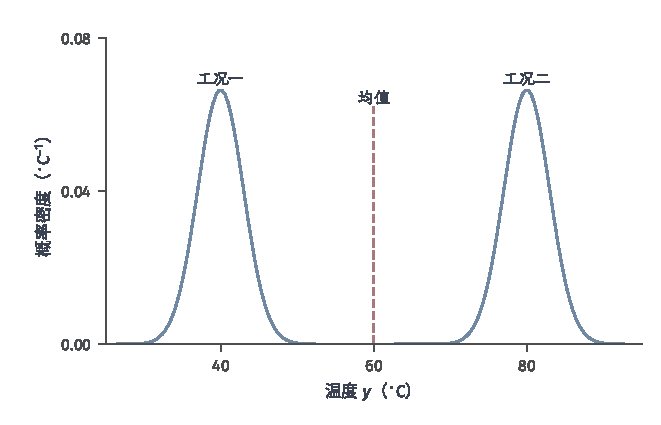
\includegraphics[width=105.412mm]{figures/06-probabilistic-graphical-models/01-representation/matplotlib/pgm-overview-predictive-density/figure.pdf}
  \caption{同一个双峰预测分布可以产生均值为$60\,^\circ\mathrm{C}$的点预测。实线为两个等权高斯密度的混合，每个分量的标准差为$3\,^\circ\mathrm{C}$；虚线标出均值。点预测没有保留两个高概率区域的位置。}
  \label{fig:pgm-overview-predictive-density}
\end{figure}

点预测和分布预测并不冲突。得到预测分布以后，仍可根据任务选择均值、概率最大的结果或其他行动。区别在于，分布先保留不确定性，点预测再按照使用目的把它压缩成一个结果。

困难在于，多个变量的联合分布会迅速变大。若有$d$个二值变量，完整联合表包含$2^d$个状态，需要$2^d-1$个自由参数。变量增多以后，有限数据很难覆盖所有组合，计算一个变量的边缘概率也可能需要汇总大量状态。概率图模型并没有取消这些困难，而是试图利用可信的局部依赖减少需要表示和计算的内容。

最强的简化是假设所有变量相互独立，但这会删掉故障与报警之间真正有用的联系。更合适的做法是只删除在特定条件下已经多余的依赖。例如，设备是否报警可以依赖是否过热和传感器是否失灵；一旦这两个状态已经给定，故障状态不必再直接进入报警的局部概率。这样的局部假设正是图结构要记录的信息。

\section{图模型上的表示}
\label{sec:pgm-overview-representation}
\label{sec:pgm-overview-basic-concepts}

本章使用四个二值随机变量：$F$表示设备故障，$H$表示过热，$A$表示报警，$S$表示传感器失灵，值$1$表示相应事件发生，值$0$表示未发生。联合概率$p(f,h,a,s)$描述四个变量同时取给定值的可能性，其中小写字母表示对应随机变量的取值。

后续章节会在有向图、因子图、团树和缺失数据图中反复使用相近符号。图~\ref{fig:pgm-overview-visual-conventions}集中列出本部分的默认视觉约定，使读者可以先辨认对象类型，再阅读具体连接。虚线的作用最依赖上下文，因此每幅图仍会在图内或图注中说明它表示辅助对应、证据读入还是分隔边界。
\begin{figure*}[htbp]
  \centering
  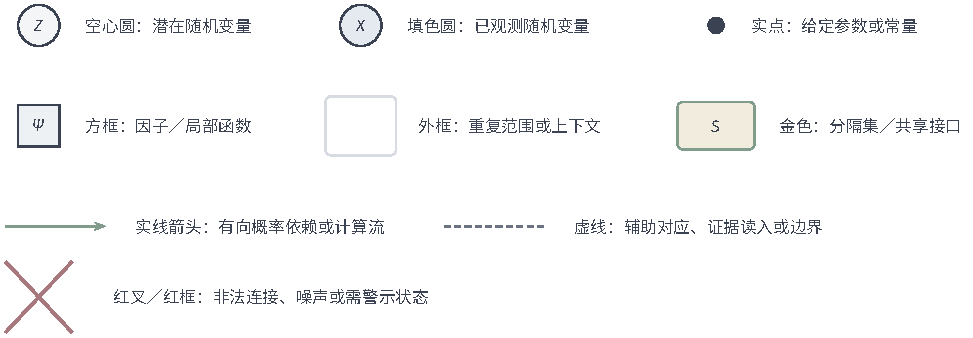
\includegraphics[width=164.747mm]{figures/06-probabilistic-graphical-models/01-representation/tikz/pgm-overview-visual-conventions/figure.pdf}
  \caption{概率图模型部分的视觉约定。空心、填色和实点区分潜变量、观测变量与给定量；方框表示局部因子，浅色填充与绿色轮廓强调团树分隔集或共享接口，红色表示非法或需警示的对象。实线箭头的概率语义与计算流语义由所在图决定；虚线只作辅助表达，不应在没有图注时自动解释为概率依赖。具体图内标注优先于本总图。}
  \label{fig:pgm-overview-visual-conventions}
\end{figure*}

汇总未知变量得到边缘分布，将证据固定并重新归一化得到条件分布。在当前设备模型中，消去未观测状态与条件化分别写为
\begin{equation}
  p(f,a)=\sum_{h,s}p(f,h,a,s),
  \qquad
  p(f\mid a)=\frac{p(f,a)}{p(a)},\quad p(a)>0.
  \label{eq:pgm-overview-marginal-conditional}
\end{equation}
这里对$h,s$求和，表示保留未知状态的所有可能性。连续变量采用相应积分。概率运算的依据参见\BookSectionRef{sec:rv-conditional-distribution}{第一卷“数学准备”的条件分布小节}。

条件独立记作$X\perp Y\mid Z$，相关等式按条件变量分布几乎处处理解。
其概率含义参见\BookSectionRef{sec:probability-moments-independence}{第一卷“数学准备”的独立关系小节}。
本部分增加的是图对这些概率约束的组织方式，以及约束如何减少联合表示和推断的成本。

联合分布总可以按变量顺序展开为条件分布的乘积，例如$p(f,s,h,a)=p(f)p(s\mid f)p(h\mid f,s)p(a\mid f,s,h)$。这条链式分解本身没有减少参数；图模型还要指定哪些条件可以删除。

在设备例子中，假设故障$F$与传感器失灵$S$独立，过热$H$只直接依赖故障，报警$A$只直接依赖过热和传感器状态。联合分布便可以写成
\begin{equation}
  p(f,h,a,s)=p(f)p(s)p(h\mid f)p(a\mid h,s).
  \label{eq:pgm-overview-device-joint}
\end{equation}
只要每个局部条件分布本身合法，这四个函数的乘积就定义了完整联合分布。对二值变量，两个根变量各需一个参数，过热条件分布需要两个，报警条件分布需要四个，总共$8$个自由参数，少于完整联合表的$15$个。减少的参数来自局部依赖假设，而不是记号上的省略。

把每个随机变量画成节点，并用箭头表示“哪个变量进入哪个局部条件分布”，就得到图~\ref{fig:pgm-overview-device-graph}。例如$H\to A\leftarrow S$对应局部项$p(a\mid h,s)$。箭头在这里记录概率分解，不凭图形本身断言因果关系。

\begin{figure}[htbp]
  \centering
  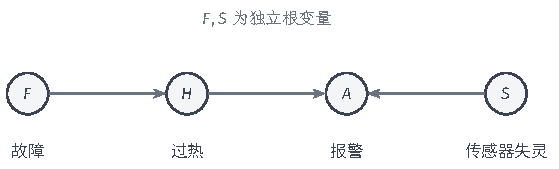
\includegraphics[width=94.590mm]{figures/06-probabilistic-graphical-models/01-representation/tikz/pgm-overview-device-graph/figure.pdf}
  \caption{设备诊断模型。节点表示随机变量，箭头指向局部条件分布所描述的变量，例如$H\to A\leftarrow S$对应$p(a\mid h,s)$。箭头指定概率分解，不自动具有因果含义。}
  \label{fig:pgm-overview-device-graph}
\end{figure}

图只说明局部依赖结构，还需要局部概率函数给出具体数值。反过来，一组数值表若没有说明各表对应哪些变量，也不足以解释整个模型。理解概率图模型时，应同时分清图结构和组成联合分布的局部函数：前者记录依赖怎样组织，后者决定模型实际给出什么概率。

图模型最基本的概率表示有两类。\term{有向图模型}（directed graphical model）像设备模型一样，用箭头组织局部条件分布；后续第~\ref{chap:pgm-directed}章将说明怎样从有向图读取条件独立关系。\term{无向图模型}（undirected graphical model）用无向边表示对称的局部相互作用，再将一组非负局部函数的乘积归一化为概率分布；第~\ref{chap:pgm-undirected}章将展开这种表示。对于局部函数$\psi_c(\bm x_c)\geq0$，写成$p(\bm x)=Z^{-1}\prod_c\psi_c(\bm x_c)$，其中$Z=\sum_{\bm x}\prod_c\psi_c(\bm x_c)$；连续情形用积分。只有$0<Z<\infty$才得到合法分布，单个势函数不必是归一化的条件概率。

\term{因子图}（factor graph）关注的是局部乘积本身。它把随机变量和局部函数画成两类节点，并在变量属于某个函数的输入时连边。因子图可以表示有向模型的条件概率乘积，也可以表示无向模型的局部函数乘积，因此它是组织计算的表示方式，不是与有向图、无向图互斥的第三类概率语义。第~\ref{chap:pgm-representations}章将比较三种表示保留的信息。比如设备模型中的$p(a\mid h,s)$可以单独画成因子节点，并连接$A,H,S$；箭头分解转换为因子图之后，乘积仍相同，但原有的父子方向不再由二部连线独自表达。这一“先分解，再画图”的理解与PRML第8章的组织一致\scite{bishop2006}

\section{图模型上的推断与学习}
\label{sec:pgm-overview-inference-learning}

图结构和局部概率确定以后，模型仍需经过计算才能回答具体问题。\term{概率推断}（probabilistic inference）是在模型已知时，根据已有证据计算所需概率。要回答“报警后设备故障的概率是多少”，需要计算$p(F=1\mid A=1)$；由于过热$H$和传感器状态$S$没有被观测，计算时必须汇总它们的所有可能取值。

把设备模型扩展到更多部件。扩展后共有$30$个未观测的二值状态，其中包括原来的过热$H$、传感器状态$S$和新增的部件状态或运行状态；以下将这$30$个未观测状态统一记为$\bm{Z}=(Z_1,\ldots,Z_{30})$。报警$A=1$仍是证据，故障$F$仍是查询目标。后验需要把这些变量的每一种配置都纳入比较：
\begin{equation}
  p(F=1\mid A=1)
  =
  \frac{
    \displaystyle\sum_{\bm{z}\in\{0,1\}^{30}}
    p(F=1,A=1,\bm{z})
  }{
    \displaystyle\sum_{f\in\{0,1\}}
    \sum_{\bm{z}\in\{0,1\}^{30}}
    p(f,A=1,\bm{z})
  }.
  \label{eq:pgm-overview-expanded-diagnosis}
\end{equation}
若直接展开，分子要汇总$2^{30}$个未观测状态配置，约为$10.7$亿项；分母还要同时遍历故障的两个取值，共有$2^{31}$个完整配置项，约为$21.5$亿项。这里的项数表示求和中需要纳入多少种状态组合，不是模型必须具有同样多的参数。

局部因子使单个完整配置$p(f,A=1,\bm{z})$通常容易评价：只需查出或计算该配置涉及的局部概率，再将它们相乘。但后验不是某个完整配置的概率，而是对大量未观测状态配置的汇总。因而，“单个完整配置易评价”和“汇总全部未观测状态仍昂贵”可以同时成立。图中的局部结构有时能够复用计算，但能节省多少取决于依赖怎样连接；具体算法与结构条件留到后续章节。

\term{精确推断}（exact inference）要求在给定模型下得到原查询的准确答案。它适合结构允许有效计算、或问题规模较小的情形；结构复杂时，中间计算仍可能非常大。\term{近似推断}（approximate inference）则在无法承担精确计算时，接受一定误差，以换取时间或空间上的可行性。第~\ref{chap:pgm-elimination}章至第~\ref{chap:pgm-sampling}章将分别展开精确与近似推断，本章不提前介绍具体实现路线。

模型中的局部概率通常不是预先知道的，还需要从数据获得。\term{参数学习}（parameter learning）在图结构和局部函数形式已经确定时，估计这些函数中的数值。例如，若记录了许多设备的故障和过热状态，就可以估计$p(H=1\mid F=1)$。数据越少、状态越稀有，估计通常越不稳定；数据中存在缺失或未观测变量时，所需计数也无法直接得到。

如果连哪些变量应直接相连也不确定，就需要\term{结构学习}（structure learning）根据数据和领域约束选择图。结构过于简单可能遗漏重要依赖，结构过于复杂则通常需要更多数据并增加计算负担。学习到有向边也不自动等于发现因果方向；因果解释需要额外假设和证据。

推断与学习解决的是不同问题：推断固定模型、计算未知状态；学习固定数据、确定模型结构或参数。当数据含有未观测变量时，两者会互相依赖，因为学习参数之前，往往要先用当前模型推断这些变量可能取什么值。第~\ref{chap:pgm-parameter-learning}和第~\ref{chap:pgm-structure-learning}章将分别展开参数与结构学习。

\section{概率图模型的历史}
\label{sec:pgm-overview-history}

概率图模型汇合了局部随机规律、条件独立语义与全局概率计算。历史中的新方法回应不同困难，没有使早期方法失去用途。图~\ref{fig:pgm-overview-history}标出代表节点，下面区分每个阶段增加了什么。

\begin{figure*}[p]
\centering
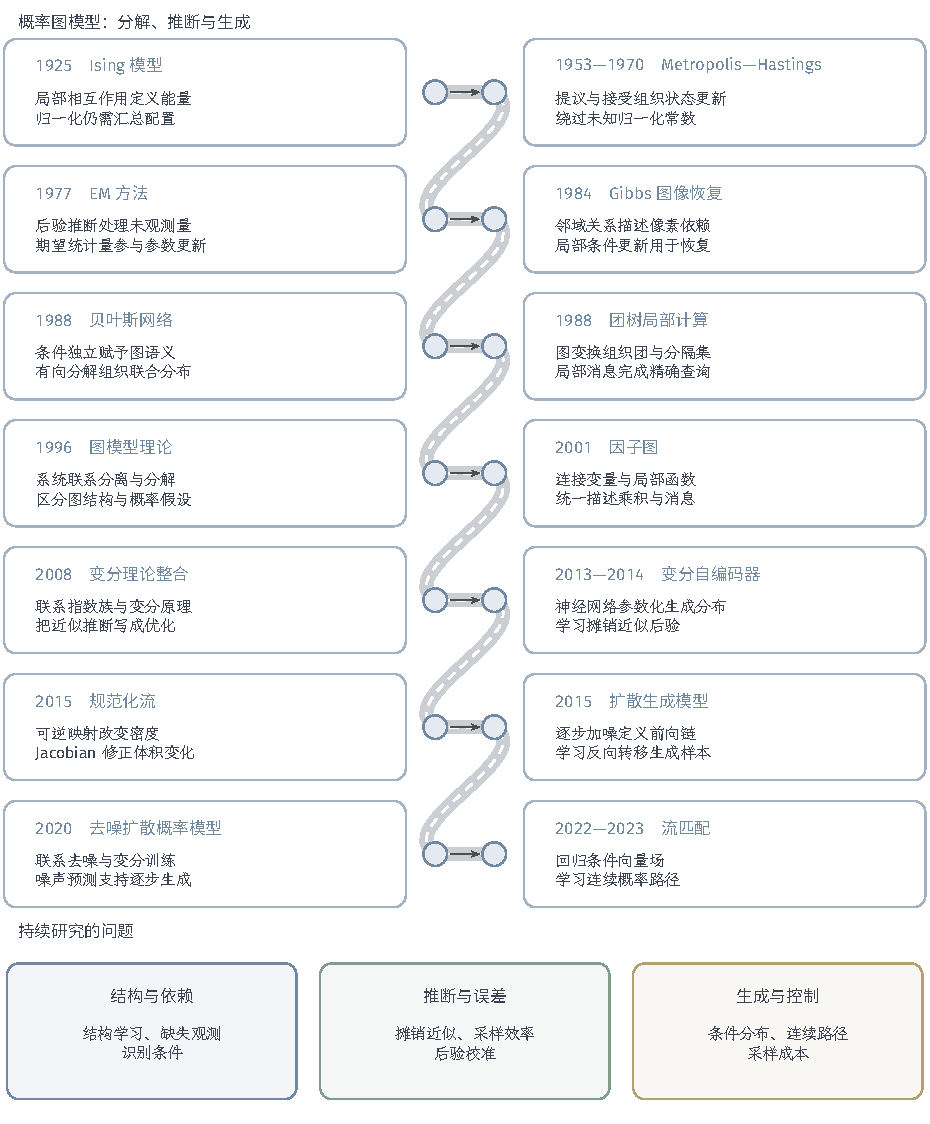
\includegraphics[width=157.406mm]{figures/06-probabilistic-graphical-models/04-models/tikz/pgm-models-history/figure.pdf}
\caption{概率图模型的代表性发展节点。局部随机模型压缩联合分布的描述，图结构提供独立性语义，推断与学习算法处理未观测量及计算困难，神经参数化再扩展局部函数与生成路径。2008年的节点表示变分理论的系统整合，并非变分推断的起源；年份对应所列代表工作，节点间距不表示实际时间长度。}
  \label{fig:pgm-overview-history}
\end{figure*}

\subsection{从局部随机规律到图结构语义}

1925年的Ising模型用相邻自旋的相互作用描述整体配置，是无向局部随机模型的早期代表。局部项压缩了模型描述，却不保证归一化和边缘概率容易计算。1977年的EM方法则处理未观测变量，使推断出的统计量参与参数更新\scite{pgm-overview-ising1925,pgm-overview-dempster1977}

当归一化常数难以计算时，可以直接围绕状态更新设计计算。1953年的Metropolis方法及1970年的Hastings推广，通过提议与接受构造随机轨迹，使未知归一化常数在接受比中消去；这条路线是否能有效估计查询，还取决于链的混合行为。1984年的Geman与Geman把局部相互作用定义的Gibbs分布与随机更新用于图像恢复，展示了局部依赖如何同时参与模型描述与计算\scite{pgm-history-metropolis1953,pgm-history-hastings1970,pgm-history-geman1984}。

1988年Pearl对概率网络的系统论述，将条件独立与有向分解联系起来；同年Lauritzen与Spiegelhalter把图变换与局部消息组织为一般网络上的精确计算方法。1996年Lauritzen进一步系统整理图模型理论。图的语义与推断算法由此可以分开判断：合法分解仍可能具有昂贵的全局查询\scite{pgm-pearl1988,pgm-overview-lauritzen1988,pgm-lauritzen1996}

\subsection{学习、近似推断与神经参数化}

模型规模增长后，变分方法把难以后验改成受限族中的优化，采样方法用随机轨迹估计查询；误差分别受近似族、优化与混合行为影响。Wainwright与Jordan在2008年的综述联系了指数族、变分原理和图上计算\scite{pgm-wainwright2008}

2013年以来，VAE用神经网络组织生成分布与近似后验，规范化流用可逆变换构造密度，扩散模型学习逆转人为噪声过程。局部函数更灵活之后，似然评价、后验近似和生成成本仍须分别处理\scite{kingma2013,pgm-overview-rezende2015,pgm-overview-sohl2015}

\subsection{当前研究方向}

一类研究在高表达能力下控制推断代价，例如设计可利用的分解结构、学习摊销后验，并检查近似误差和校准。另一类将神经生成模型用于高维条件分布，比较潜变量、可逆变换、扩散与连续流的表示和采样成本。流匹配通过拟合条件向量场学习连续生成路径，是这一方向的代表方法\scite{lipman2023flowmatching}

面向不完整、多模态或有领域约束的数据，还需让结构假设、识别条件与预测查询相容。研究热点不能仅按生成质量排序：模型是否保留目标依赖、训练能否找到合适参数、有限数据下预测是否可靠，仍是三个独立问题。

\section{本章小结}
\label{sec:pgm-overview-summary}

点预测给出一个结果，概率分布则保留其他结果的可能性。多个变量的联合分布会随变量数量迅速增大，概率图模型因此用局部条件独立组织依赖，再由局部概率函数组成联合分布。图结构减少了需要明确指定的关系，但这种简化是否成立，取决于局部假设是否符合问题。

图模型上的表示以有向图和无向图为两种基本概率语义，因子图则把两类模型中的局部乘积显式画出来。局部因子可以让单个完整配置易于评价，却不保证汇总大量未观测状态配置同样容易。模型给定后，推断根据证据回答概率查询；数据给定后，学习估计参数或选择结构。

表示、计算和学习上的困难共同推动了概率图模型的演进：局部随机规律压缩依赖，图结构赋予这些依赖可检查的语义，精确推断重组全局计算，学习与近似推断处理未知模型和不可承受的查询，神经参数化再扩展局部函数的表达能力。这些路线各有边界，没有按时代相互取代。下一章将从有向图出发，严格说明图结构、条件独立和联合分解怎样联系起来。

\paragraph{扩展阅读}
Bishop的PRML第8章从局部概率分解解释图的意义，Koller与Friedman的教材系统区分表示、推断和学习。阅读时可持续用同一个查询核对图结构节省了哪一种表示或计算\scite{bishop2006,pgm-koller2009}
